%  LaTeX support: latex@mdpi.com 
%  In case you need support, please attach all files that are necessary for compiling as well as the log file, and specify the details of your LaTeX setup (which operating system and LaTeX version / tools you are using).

% You need to save the "mdpi.cls" and "mdpi.bst" files into the same folder as this template file.

%=================================================================
\documentclass[sensors,article,submit,moreauthors,pdftex,10pt,a4paper]{mdpi} 


%
%--------------------
% Class Options:
%--------------------
% journal
%----------
% Choose between the following MDPI journals:
% actuators, admsci, aerospace, agriculture, agronomy, algorithms, animals, antibiotics, antibodies, antioxidants, applsci, arts, atmosphere, atoms, axioms, batteries, behavsci, beverages, bioengineering, biology, biomedicines, biomimetics, biomolecules, biosensors, brainsci, buildings, carbon, cancers, catalysts, cells, challenges, chemosensors, children, chromatography, climate, coatings, computation, computers, condensedmatter, cosmetics, cryptography, crystals, data, dentistry, designs, diagnostics, diseases, diversity, econometrics, economies, education, electronics, energies, entropy, environments, epigenomes, fermentation, fibers, fishes, fluids, foods, forests, futureinternet, galaxies, games, gels, genealogy, genes, geosciences, geriatrics, healthcare, horticulturae, humanities, hydrology, informatics, information, infrastructures, inorganics, insects, instruments, ijerph, ijfs, ijms, ijgi, ijtpp, inventions, jcdd, jcm, jdb, jfb, jfmk, jimaging, jof, jintelligence, jlpea, jmse, jpm, jrfm, jsan, land, languages, laws, life, literature, lubricants, machines, magnetochemistry, marinedrugs, materials, mathematics, mca, mti, medsci, medicines, membranes, metabolites, metals, microarrays, micromachines, microorganisms, minerals, molbank, molecules, mps, nanomaterials, ncrna, neonatalscreening, nutrients, particles, pathogens, pharmaceuticals, pharmaceutics, pharmacy, philosophies, photonics, plants, polymers, processes, proteomes, publications, recycling, religions, remotesensing, resources, risks, robotics, safety, sensors, separations, sexes, sinusitis, socsci, societies, soils, sports, standards, sustainability, symmetry, systems, technologies, toxics, toxins, tropicalmed, universe, urbansci, vaccines, vetsci, viruses, water
%---------
% article
%---------
% The default type of manuscript is article, but can be replaced by: 
% addendum, article, book, bookreview, briefreport, casereport, changes, comment, commentary, communication, conceptpaper, correction, conferenceproceedings, conferencereport, expressionofconcern, meetingreport, creative, datadescriptor, discussion, editorial, essay, erratum, hypothesis, interestingimage, letter, newbookreceived, opinion, obituary, projectreport, reply, retraction, review, preprints, shortnote, supfile, technicalnote
% supfile = supplementary materials
%----------
% submit
%----------
% The class option "submit" will be changed to "accept" by the Editorial Office when the paper is accepted. This will only make changes to the frontpage (e.g. the logo of the journal will get visible), the headings, and the copyright information. Also, line numbering will be removed. Journal info and pagination for accepted papers will also be assigned by the Editorial Office.
%------------------
% moreauthors
%------------------
% If there is only one author the class option oneauthor should be used. Otherwise use the class option moreauthors.
%---------
% pdftex
%---------
% The option pdftex is for use with pdfLaTeX. If eps figure are used, remove the option pdftex and use LaTeX and dvi2pdf.

%=================================================================
\firstpage{1} 
\makeatletter 
\setcounter{page}{\@firstpage} 
\makeatother 
\articlenumber{x}
\doinum{10.3390/------}
\pubvolume{xx}
\pubyear{2017}
\copyrightyear{2017}
\externaleditor{Academic Editor: name}
\history{Received: date; Accepted: date; Published: date}

%------------------------------------------------------------------
% The following line should be uncommented if the LaTeX file is uploaded to arXiv.org
%\pdfoutput=1

%=================================================================
% Add packages and commands here. The following packages are loaded in our class file: fontenc, calc, indentfirst, fancyhdr, graphicx, lastpage, ifthen, lineno, float, amsmath, setspace, enumitem, mathpazo, booktabs, titlesec, etoolbox, amsthm, hyphenat, natbib, hyperref, footmisc, geometry, caption, url, mdframed

%=================================================================
%% Please use the following mathematics environments: Theorem, Lemma, Corollary, Proposition, Characterization, Property, Problem, Example, ExamplesandDefinitions, Remark, Definition
%% For proofs, please use the proof environment (the amsthm package is loaded by the MDPI class).

%=================================================================
% Full title of the paper (Capitalized)
\Title{EEG Waveform Analysis with applications to Brain Computer Interfaces}

% Authors, for the paper (add full first names)
\Author{Rodrigo Ramele $^{1,\dagger}$, Ana Julia Villar $^{1}$ and Juan Miguel Santos  $^{1}$*}
% Authors, for metadata in PDF
\AuthorNames{Rodrigo Ramele, Ana Julia Villar and Juan Miguel Santos}

% Affiliations / Addresses (Add [1] after \address if there is only one affiliation.)
\address[1]{%
$^{1}$ \quad Computer Engineering Department, Instituto Tecnológico de Buenos Aires (ITBA); info@itba.edu.ar}

% Contact information of the corresponding author
\corres{Correspondence: rramele@itba.edu.ar; Tel.: +54-9-11-4193-9382}

% Current address and/or shared authorship
\firstnote{Current address: C1437FBH Lavarden 315, Ciudad Autónoma de Buenos Aires, Argentina} 

% Simple summary
%\simplesumm{}

% Abstract (Do not use inserted blank lines, i.e. \\) 
\abstract{The Electroencephalography is not just a mere clinical tool anymore.  It has become the de-facto mobile, portable, non-invasive brain imaging sensor to harness brain information in real time and translating or decoding brain signals, detecting information that can be used to diagnose disease or implement Human Computer Interaction devices.  The traditional automatic approach which is based heavily on using digital tools to detect the cloaked information  in the signal, outshining the research done by the EEG community which was based heavily on EEG waveforms: the structure of signal plots.  The purpose of this work is to provide a bridge by doing a survey and description of the automatic methods that has been used to detect patterns in the waveforms, and to perform a benchmarking approach to determine different characteristics of those methods aiming to detect  specific waveforms mimicking what technician has been done since the inception of this fruitful technology. }

% Keywords
\keyword{electroencephalography (EEG); ERP,VEP,waveform, signal structure}

% The fields PACS, MSC, and JEL may be left empty or commented out if not applicable
%\PACS{J0101}
%\MSC{}
%\JEL{}
%\AMS{}

% If this is an expanded version of a conference paper, please cite it here: enter the full citation of your conference paper, and add $^\S$ in the end of the title of this article.
%\conference{}

%%%%%%%%%%%%%%%%%%%%%%%%%%%%%%%%%%%%%%%%%%
% Only for the journal Data:

%\dataset{DOI number or link to the deposited data set in cases where the data set is published or set to be published separately. If the data set is submitted and will be published as a supplement to this paper in the journal Data, this field will be filled by the editors of the journal. In this case, please make sure to submit the data set as a supplement when entering your manuscript into our manuscript editorial system.}

%\datasetlicense{license under which the data set is made available (CC0, CC-BY, CC-BY-SA, CC-BY-NC, etc.)}

%%%%%%%%%%%%%%%%%%%%%%%%%%%%%%%%%%%%%%%%%%
% For Conference Proceedings Papers: add the conference title here
%\conferencetitle{}

%\setcounter{secnumdepth}{4}
%%%%%%%%%%%%%%%%%%%%%%%%%%%%%%%%%%%%%%%%%%
\begin{document}

%%%%%%%%%%%%%%%%%%%%%%%%%%%%%%%%%%%%%%%%%%
%% Only for the journal Gels: Please place the Experimental Section after the Conclusions

%%%%%%%%%%%%%%%%%%%%%%%%%%%%%%%%%%%%%%%%%%
\setcounter{section}{-1} %% Remove this when starting to work on the template.

\section{Introduction}

Current society is demanding technology to once and for all provide the means to realize the utopia of social inclusion for people with disabilities.  At the same time, a worldwide aging population is also asking for means to extend active lifestyles throughout all life, including the extending years that medicine is allowing us to have.
Finally, our digital gadgets and the digital revolution have modified the way we interact with all our devices.  A new emerging digital society is consolidating: smart wearable health sensors are required to implement automatic detection of situatedness or detecting health activities, in an active or passive way.
All our communication with devices is based on movement (introduction gauger state of the art 7), but all these trends are precisely pushing this boundary beyond the limitation of our body, beyond the limitation of our own movement.  A new form of Human Machine Interaction was needed and this is how Brain Machine Interfaces were born.  Moreover, as long as we keep putting computer inside every machine (REF IOT), this will be not other thing that Brain Computer Interfaces (BCI).
In the center of all this hype, we can find a hundredth year old technology, rock-solid as a diagnosis tool, which greatly benefited from the shrinkage of sensors, computer power, wireless protocols and advanced electronics: the Electroencephalogram (EEG).

EEG sensors are wearable (Sensors EEG Review, TOward mobile EEG), non-invasive, portable and mobile, with excellent temporal resolution, and acceptable spatial resolution (EEG Patterns).  This humble diagnosis device has been transformed into  currently the best approach that we have to precisely detect, out-of-the lab, information from the Brain, directly from the source of volition (footnote), and to use that information to drive our cars, steer our drones, write our emails, and control our wheelchairs (references of everything)

The traditional approach to analyze EEG signals were based on detecting visual patterns out of the EEG trace or polygraph (Atlas of EEG patterns): analog and reference signals were extracted and plotted over a piece of paper, continuously. Electroencephalographers or Electroencephalography technician have decoded and detected patterns in the signals by visually inspecting the signals.  Moreover, clinically, nowadays EEG remains a visually interpreted test (ATLAS EEG)

With the development of automatic electronics, first analog electronic devices and later computarized digital processing methods, mathematically and algorithmically complex procedures were established to decode the information with incredible success.

However, the traditional and knowledgeable approach was mainly overshadow, and the waveform of the EEG was replaced by a black box approach.

The aim of this study is threefold: first  to review current literature of EEG processing techniques which are based on analysis of the waveform.  The second is to evaluate and study the methods by analyzing its performance against a pseudo-real dataset. We aim to provide a better understanding of the different approaches.  We believe that the importance of the waveform analysis methods, as described here, is that by using these kind of approaches colaboration is fostered because there is a clear description and characterization of the signal and the extensive literature which explores EEG can be reviewed from the same point of view. 

Enhancing this bridge will be beneficial to both ends: connections between BCI community and other communities (ref Nijboer, BCI a Review), and at the same time an automatic approach to empower what technician regularly do in EEG diagnosis.

BCI REsearch is 71.2 percent based on EEG (recent advancent summary 2016)

We believe that studying specific componentes may lead to better understanding of the neuro component.

%Novel sensor design and smart embodiment for pervasive healthcare;
%New platforms for self-tracking or measurement of physical activity, sleep quality, emotion, gait, kinematics, kinetics and other factors related to personal well-being;
%Information processing for localization and tracking for healthcare applications
%Resource constrained network information processing for healthcare applications
%Sensor data analytics, information integration, pattern mining/recognition, behaviour profiling, data visualisation and user feedback related to personal well-being;
%
%Mobile/wearable sensor-based/remote health monitoring systems, with illustrative case studies on use of innovative information processing approaches.
%Disease focused exemplars and case studies (e.g. neurological disorders, cardiovascular diseases, diabetes and obesity, neuro-rehabilitation);

\section{Electroencephalography Waveform Analysis}

distinguishing the pertinent signal characteristics from extraneous content and representing them in a compact or menaingful form, amenable to interpretation by a human or computer (Wolpaw and Wolpaw)


Shape or waveform analysis methods are considered as nonparametric methods (in opposition to statistical or dynamical models).  They can explore the amplitude, energy, teager energy operand, or more complex like the L-Z Lempel-Ziv complexity measurement (thakor qEEG).


The Electroencephalogram is one of the most widespread used device to capture brain signals.  It was initially developed by Hans Berger and has been extensively used for decades to diagnose neural diseases and other medical conditions.

The first thing that he saw was the visual cortical alpha wave characterization, the Berger Rythm.  Its amplitude and power determine that this feature can be coherently assosiated to a cognitive phenoma (eyes closed).  We should ask ourselves if the EEG should be described years later if this particular event wasn't so evident.

The EEG signal is not stationary, highly complex.  It can be characterized as a linear stochastic process with great similarities to noise (Thakor EEG).  They are measured in microvolts.
they have many artifacts.

The most important part to consider is that of montage.  It could be bipolar or referencial.  In general EEG can be rereferenced offline.The traditional convention, somehow maintained in neuro research, downward polarity was considered negative and upward deflection for negative (Knott, 1985)  It is of utmost importance to remark that  EEG waveforms repre- sent the differential voltage between a given electrode and the recording reference. It is therefore clear that the choice of reference completely determines EEG wave- forms (Lehmann, 1987; Dien, 1998), an important method- ological consideration that all too often is still not recog- nized in the EEG literature. For example, recording with a vertex (Cz) reference would lead to small EEG deflections in the proximity of Cz due to potential synchronization of firing activities within closely spaced brain regions and vol- ume propagation of the EEG signal. Similarly, recording with mastoid or linked ears montage would lead to rather small waveforms at electrodes positioned over temporal brain regions (Pivik et al., 1993).

The automatic processing of EEG signals can be called qEEG is precisely the opposite of what we are doing here, quantite analysis (OJO)

The conventional clinical method of observing the waveform is thought to be subjective and laborius because the results depend on the technicians' experience and expertise.  This call for objective measurements pushed the adoption of qEEG methods and the need for automation (Thakor qEEG)


Some initial works on EEG explored the idea to extend human capacities analyzing EEG waveforms  (automatic detection of k complexes), (A Waveform Analyzer Applied to the Human EEG) where a feature from amplitude and frequency of its signal and its derivative in time-domain is used.  Althought CASENET REFERENCe explored "waveform" structure they were purely based on spike detection based on feeding artificial neural networks.  It is likeyly that the Matched Filter approach (linear) gave poor results and nonlinear methods based on neural network were being explored.It has been the traditional approach for technician, but the advent of elecrical processing, more sophisticated methods.


EEG has been used extensively on Sleep Research, by performing Polysomnographic recordings (PSG)  (reference of the german paper of Sleep Research) where scoring of EEG to determine different sleep stages were performed by visually marking waveforms or graphoelements looking for patterns based on standardized guidelines.

Visual characterization includes the identification or classification of componentes, or transient events, based on phase, monophasic or biphasic  (i.e. positive and negative component) where different components are measured, relation between them is stablished and index are created (e.g. sleep K-Complex is well characterized based on relation rates between positvie vs negative amplitude) (REFERENCE).  Relevant EEG patterns for sleep stage scoring are alpha, theta, and delta waves,
sleep spindles, polysplindles, K-complexes, vertex sharp waves (VSW), and sawtooth waves (REM Sleep)


Transient phenomena allows also to record occurrence and temporal sequence (mimicking spike analysis in neuro reserach)

The traditional approach do not consider waveform even though the brain oscilations are in general nonsinusoidal (reference)

This approach is relative common in chemical analysis (i.e. chemometrics Skoog, D.; West, D.; Holler, F. Analtyical Chemistry, An Introduction; Saunders: Philadelphia, 1994.), geology (sismic analysis), and quantitive financial analysis.  EKG, or Electrocardiogram, on the other hand, has been extensively processed and analyzed by waveform methods.



Slight variations in whether slopes or other features are scored may be important to certain applications.

waveform, phase, amplitude and frequency

waveform amplitud plotted against time

characteristic shape, or waveform.
rising phase
falling phase
pronounced plateau
ripples, wiggles, 

P,Q,R,S,T peaks in EKG analysis (REFERENCE) 

aEEG, amplitude integrated electroencephalography or cerebral function monitoring (REFERENCE)

Artefacts: endogeneous exogeneous
Non-Stationarity: this means that this and that.  What does it mean in terms of the signal.
DC drift and trending
Basal EEG activity

Inter-subject and intra-subject variability

Non-exhaustive list of transient events

Determination of transient events, and particularly amplitude of different subcomponents, latency or even phase, has proved very importan concequences in terms of the different cognitive approach.

Rhythms in neural activity are observed across various temporal and spatial scales and are often
referred to as oscillations (see Glossary) [1]. Traditionally, neural oscillations have been
clustered into canonical frequency bands, including delta (1–4 Hz), theta (4–8 Hz), alpha (8–
12 Hz), beta (15–30 Hz), gamma (30–90 Hz), and high gamma (>50 Hz). These bands roughly
correspond to frequency ranges commonly observed in human electroencephalography (EEG)
studies. Although they have been observed for nearly a century, recent theories suggest that
these oscillations play an active role in neural communication


 Hippocampal theta oscillations, for example, are among
the best-studied rhythms in the local field potential (LFP); they have a stereotyped sawtooth
shape

Standard signal processing characterization (chemical, time series reference, sismic reference) can also be applied.


EEG is a multidimensional signal non-stationary 

Amplitude
Arch
Frequency
Phase
Nonsinusoidal sinusoidal
Oscilation
Sawtooth: motor cortical beta oscillations
Sharpness
Spike-wave discharge
Transient event

inverse problem is mathematically intractable Voytek 2009

Brainwaves may be missleading because what is actually been harnessed is electrical potentials over the scalp

Reference to the good paper about how EEG actually works

(Paper de Spinelli) 

CFC, Cross Frequency Coupling, sharper, arch comb or wicket shape, sawtooth, rectangular, spike-wave like, decay phase, voltage rise, peaks and troughs, short term voltage change around each extrema in the raw trace, peak and trough sharpness ratio, symmetry between rise and decay phase, slope ratio (steepness of the rise period to that of the adjacent decay period.

Central trough is sharper and more negative that the adjacent troughs.

Phase-Amplitude Coupling, Phase-Phase Coupling.


Dimensionality reduction which is truly applied when the waveform is actually formed

Oscillatory activity can also have their differente or distinctive waveforms.  Slow oscillations, which are assosiated with REM, sawtooth-shaped.
Sleep spindles can also be considered oscilations and they have a distintinc form assosiated with stage 2 dream.
Visual Cortical alpha and rolandic central mu waves arch-like structure (similar to the greek letter mu).  Slope Ratio.  Trough voltage remains contstant while peak voltage fluctuates.   Steep slopes,   Amplitude asymmetry 
ponto-geniculo-occipital
(PGO) waves

In sleep research sleep 2 stage the background of KComplex and sleep spindles is theta waves

Another approach which is very related to EEG waveform analysis is the detection of latency, amplitude and phase components in ERP.  It is known that these characteristics can be mapped to cognitive or disease situations.  We hypothesize that that including more approaches can lead to a better understanding or opening of a new field.

by application to Brain Computer Interfaces or EEG diagnosis (BCI a review, BCI Vidal 1973)

Seizures captured in their entirety typically show progression from low-voltage, high-frequency spikes to high-voltage, low-fre- quency spike-and-slow wave activity, before stopping abruptly and being replaced by background slowing or suppression (Fig. 29.9). Usual morphologic features include typical rhythmic, gen- eralized, symmetric spike-and-waves or polyspikes and waves at 2 to 3.5 Hz; atypical spike and wave with lower frequency and less symmetry; multiple spike-and-wave (repetitive complexes of two or more spikes followed by a slow wave); and high-voltage, repetitive, rhythmic, focal or generalized delta activity with inter- mixed spikes, sharp waves, or sharp components (Fig. 29.24) (45). Diagnosis is more difficult when the seizure (or SE) pre- cedes the beginning of the tracing and continues beyond its end. In such cases, rhythmic sharp features, typically faster than 1 Hz, may be seen, often with variability.

(e.g. FIRDA - Frontal Intermittent Rhythmic Delta) and posteriorly in children e.g. OIRDA - Occipital Intermittent Rhythmic Delta).

alpha dissapears when alerting by any mechanism (thinking, calculating)


Rhythmic. EEG activity consisting in waves of approximately constant frequency.
Arrhythmic. EEG activity in which no stable rhythms are present.
Dysrhythmic. Rhythms and/or patterns of EEG activity that characteristically appear in patient groups or rarely or seen in healthy subjects.

Attenuation (synonyms: suppression, depression). Reduction of amplitude of EEG activity resulting from decreased voltage. When activity is attenuated by stimulation, it is said to have been "blocked" or to show "blocking".

Hypersynchrony. Seen as an increase in voltage and regularity of rhythmic activity, or within the alpha, beta, or theta range. The term implies an increase in the number of neural elements contributing to the rhythm. (Note: term is used in interpretative sense but as a descriptor of change in the EEG).
Paroxysmal. Activity that emerges from background with a rapid onset, reaching (usually) quite high voltage and ending with an abrupt return to lower voltage activity. Though the term does not directly imply abnormality, much abnormal activity is paroxysmal.


Monomorphic. Distinct EEG activity appearing to be composed of one dominant activity

Polymorphic. distinct EEG activity composed of multiple frequencies that combine to form a complex waveform.

Sinusoidal. Waves resembling sine waves. Monomorphic activity usually is sinusoidal.

Transient. An isolated wave or pattern that is distinctly different from background activity.

a) Spike: a transient with a pointed peak and a duration from 20 to under 70 msec.
b) Sharp wave: a transient with a pointed peak and duration of 70-200 msec.



generalized, focal or lateralized.

Artifact detection and averaging.


\section{Materials and Methods}

%To verify the validity of the proposed framework and method, the public dataset 008-2014  \citep{Riccio2013} published on the BNCI-Horizon website \citep{Brunner2014} by  IRCCS Fondazione Santa Lucia, was used to perform a binary classification task on the provided signals.  The algorithm was implemented using the VLFeat  \citep{Vedaldi2010} Computer Vision libraries on MATLAB 2014a (Mathworks Inc., Natick, MA, USA). 

In order to determine which  processing method to be considered as a  "waveform template matching" we restrict ourselves to the following criteria:

\begin{itemize}
\item The pattern can be identified and verified by visual inspection.
\item The pattern matching is performed in time-domain.
\item The analysis take account the shape of the plot of the signal.
\item They can be used as templates.
\item Transient events ?
\item Single Channel
\end{itemize}

Although the term morphology has been used to identify this approach, We specifically excluded morphological based methods
\cite{Yamaguchi2009}.  On the other hand, Morphological Component Analysis is a variant form of Blind Source Separation which can be considered the extension of Matching Pursuit algorithm. (cita a esa parte del paper).

As described in (Mixed Domain Signal Analysis) the Pattern Matching problem in Signal processing is finding a signal given the region that best describes the structure of the pattern.

\subsection{Peak Picking}

The name of many of the EEG features reference indeed peaks like P300 or P3a P3b or N100.   This leads to a natural way to classify them visually by selecting appropiate peaks and matching their positions and amplitudes in an orderly manner.

Although of limited usability, peak picking is the first automatic method of detection and has been used to determine latency of transient events in EEG.  Straighforward in its implementation, it consist in selecting a component, particularly a simple component based on the expected location of its more prominent deflection.

Ouyang2017,Zhang2011

difference of areas (trabajo Mexicanos)

 integrated activity (area measure) (area measure)
 
 It was used in Farwell and Donchin work on P300 (Wolpaw and Wolpaw).

\subsection{Woody's Template Matching}

Cross Covariance with Template or Cross Correlation

Applying a FIR filter with templates 

Krusienski et al 2007
Serby et al 2005

extended to wavelent analysis.

\subsection{Matching Pursuit}

Pursuit algorithms refer, in their many variants, as blind source separation techniques that assume that the EEG signal is a linear combination of different sources that comes from template dictionaries.

We include them here because they are traditional in terms for the traditional view of Morphological Analysis or Shape domain analysis, though they do not restrict to our own definition of "shape domain processing".

However in terms of 

\subsection{Dynamic Time Warping}

Dynamic Time Warping is a technique 

\subsection{Wrapping Method}

\subsection{Permutation Entropy}

Bond and Pompe PE method.

\subsection{ACF: Autocorrelation Function}

\subsection{Waveform Complexity}

Lempel-Ziv method L-Z complexity

\subsection{Slope Horizontal Chain Code}

contour representation based on an adapted version of the Slope Chain Code (SCC)

\subsection{Warp Averaging}

%\subsection{Morphological Signal Analysis}
%
%Several approaches and methods have been applied to decode them.  Of particular interests are morphological signal analysis 
%CITE (Paper del chabon del ITBA que detalla bien los diferentes metodos) \citep{Alvarado-Gonzalez2016,Yamaguchi2009}.
%
%Morphological or 
%
%template matching
%
%spike
%sharp wave
%spike wave
%polyspike 
%slow wave complex
%
%shape domain
%
%\subsection{P300}
%
%Uhhhh I can talk a lot about P300 \citep{Knuth2006}.
%
%P300 single trial is a golden grail of Brain computer interfaces.  It is studied and analyzed in this way, here in this other way, in this other way is here.

\subsection{EEG based on Histogram of Gradients}

\subsection{Experimental Protocol}

In order to verify each one of the approaches we will inject into a known dataset spurious p300 signal that we may be able to control.  By implementing this pseudo-real approach, we can effectively control null-signals of this evoked potentials following the same approach of other similar works ( ref   Ouyang2017, el trabajo de estudio de templates y el trabajo de p3).

At the same time adding a mixed signal with varying degrees of SNR will allow us to determine robustness of the different methods.

The second part, we will specifically find the P300 signal from a dataset.

amplitude
latency

in a single trial approach.  The template was obtained from the point to point average of a standard p300 experiment (published elsewhere).

The original signal-to-noise ratio was calculated as Hue 2010 as 

\begin{itemize}
\item Peak Finding
\item Woody Template Matching
\item Permutation Entropy
\item SHCC (los mexicanos me dijeron que me dan el codigo para matlab)
\item BCI SIFT
\end{itemize}

\begin{itemize}
\item Inyectar una señal en un tren de EEG simulando el P300
\item Probar con diferentes metodos la capacidad de detectar si un segmento contiene o no el patron
\item Probar con diferentes metodos la capacidad de identificar correctamente la localizacion del patron.
\item Probar variando la señal relacion ruido usando la formula de Huo y con eso ver como cada metodo permite mantenerse.
\end{itemize}






%The central part of this method is the feature generation: the histogram of image gradients.  To do so, the first step is the transformation of the signal into a temporary binary image.
%
%The signal is first scaled and centered at zero by 
%
%\begin{equation}
%\tilde{x}(t,c) = \left \lfloor{ \gamma \cdot ( x(t,c) - \bar{x}(t,c)  )}\right \rfloor
%\end{equation}
%
%\noindent where $\gamma$ is the image scale, $t$ is time and $ x(t,c) $ is the EEG matrix defined for each $t$ and for a particular channel $c$.
%
%Then the image is constructed by
%
%\begin{equation}
%I(z_1,z_2) = \left\{ \begin{array}{rl}
%255 & z_1 = \gamma \cdot t; z_2 = \tilde{x}(t,c) + z(c) \\
%0   & \mbox{otherwise}
%\end{array}\right.
%\label{eq:images}
%\end{equation}

BLABLABLABLA \ref{fig:sampledescriptor}.
 
\begin{figure}[H]
\centering
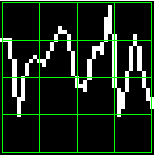
\includegraphics[width=6cm]{sampledescriptor.png}
\caption{The local patch is located around a sample point plotted on the temporary image. All the sample points are interpolated using the Bresenham algorithm. The 4x4 block grid can be seen on the patch as well as the green arrows showing the dominant gradient on each block.}
\label{fig:sampledescriptor}
\end{figure}


\subsubsection{Classification}

In order to classify we will use the same classifier for every method.  By doing this we will avoid 


\subsubsection{Parameters}

BLABLALBALBALBAL

%%%%%%%%%%%%%%%%%%%%%%%%%%%%%%%%%%%%%%%%%%
\section{Results}
\label{section:results}
sections

BLABLABLABLALBA


\begin{table}[H]
\caption{Accuracy levels obtained by a 3-fold cross validation. The values reported by the dataset publishers for Cz are reproduced here for comparison. Additionally, BCI accuracies for channel Cz can be seen as well as performance levels and their standard deviation obtained for the BPC, the best performing channel for each subject.}
\centering
%% \tablesize{} %% You can specify the fontsize here, e.g.  \tablesize{\footnotesize}. If commented out \small will be used.
\begin{tabular}{ccccc}
\toprule
\textbf{Participant}	& \textbf{Original Cz}	& \textbf{ACC at Cz}	& \textbf{BPC}	& \textbf{Performance}\\
\midrule
1     &   0.84 &   0.79 & Cz  &   0.79 $\pm$ 0.01 \\
2     &   0.86 &   0.81 & PO7 &   0.93 $\pm$ 0.01 \\
3     &   0.87 &   0.78 & Cz  &   0.78 $\pm$ 0.03 \\
4     &   0.86 &   0.68 & PO8 &   0.90 $\pm$ 0.01 \\
5     &   0.86 &   0.80 & PO7 &   0.93 $\pm$ 0.01 \\
6     &   0.89 &   0.96 & Cz  &   0.96 $\pm$ 0.01 \\
7     &   0.89 &   0.78 & PO7 &   0.93 $\pm$ 0.01 \\
8     &   0.92 &   0.91 & PO7 &   1.00 $\pm$ 0.00 \\
1     &   0.84 &   0.81& Fz&   0.82 $\pm$ 0.0017 \\
2     &   0.86 &   0.82& Fz&   0.85 $\pm$ 0.0011 \\
3     &   0.87 &   0.82& Cz&   0.82 $\pm$ 0.0011 \\
4     &   0.86 &   0.81& PO7&   0.82 $\pm$ 0.0012 \\
5     &   0.86 &   0.82& Fz&   0.82 $\pm$ 0.0021 \\
6     &   0.89 &   0.81& Fz&   0.82 $\pm$ 0.0016 \\
7     &   0.89 &   0.83& Fz&   0.84 $\pm$ 0.0011 \\
8     &   0.92 &   0.82& PO7&   0.84 $\pm$ 0.0020 \\
\bottomrule
\end{tabular}
\label{tab:results}
\end{table}

%%%%%%%%%%%%%%%%%%%%%%%%%%%%%%%%%%%%%%%%%%
\section{Discussion}

BLABLABLABLABLALBA


This method, different from other methods which is based on the nonlinearity of the gradient of histograms which can be used to detect 

is also based on how the image look like.

SNR of p300 and how to detect it

Check if you can use this to detect any kind of transient signal.

Compare if it is possible with the descriptors from one subject, discriminate the others.

Channal identification based on the metric distance between the bags


%%%%%%%%%%%%%%%%%%%%%%%%%%%%%%%%%%%%%%%%%%
\section{Conclusion}



%%%%%%%%%%%%%%%%%%%%%%%%%%%%%%%%%%%%%%%%%%
%\subsection{Subsection}
%
%\subsubsection{Subsubsection}
%
%Bulleted lists look like this:
%\begin{itemize}[leftmargin=*,labelsep=4mm]
%\item	First bullet
%\item	Second bullet
%\item	Third bullet
%\end{itemize}
%
%Numbered lists can be added as follows:
%\begin{enumerate}[leftmargin=*,labelsep=3mm]
%\item	First item
%\item	Second item
%\item	Third item
%\end{enumerate}
%
%The text continues here.



%%%%%%%%%%%%%%%%%%%%%%%%%%%%%%%%%%%%%%%%%%
\vspace{6pt} 

%%%%%%%%%%%%%%%%%%%%%%%%%%%%%%%%%%%%%%%%%%
%% optional
%\supplementary{The following are available online at www.mdpi.com/link, Figure S1: title, Table S1: title, Video S1: title.}

%%%%%%%%%%%%%%%%%%%%%%%%%%%%%%%%%%%%%%%%%%
\acknowledgments{This project was supported by the ITBACyT-15 funding program issued by ITBA University.}

%%%%%%%%%%%%%%%%%%%%%%%%%%%%%%%%%%%%%%%%%%
\authorcontributions{This projects is part of a the first author's PhD Thesis which is directed by Juan Miguel Santos and codirected by Ana Julia Villar.}

%%%%%%%%%%%%%%%%%%%%%%%%%%%%%%%%%%%%%%%%%%
%\conflictofinterests{The authors declare no conflict of interest.} 

%%%%%%%%%%%%%%%%%%%%%%%%%%%%%%%%%%%%%%%%%%
%% optional
\abbreviations{The following abbreviations are used in this manuscript:\\

\noindent EEG: electroencephalography\\
BCI: Brain Computer Interfaces\\
SNR: Signal to Noise Ratio\\
CNS: Central Nervous System\\
ALS: Amyotrophic Lateral Sclerosis\\
ERP: Event-Related Potential\\
P300: Positive deflection of an Event-Related Potential which occurs 300 ms after onset of stimulus\\
ITR: Information Transfer Rate\\
BTR: Bit Transfer Rate\\
SIFT: Scale Invariant Feature Transform\\
HOG: Histogram Of Gradients}

%%%%%%%%%%%%%%%%%%%%%%%%%%%%%%%%%%%%%%%%%%
%% optional
%\appendixtitles{no} %Leave argument "no" if all appendix headings stay EMPTY (then no dot is printed after "Appendix A"). If the appendix sections contain a heading then change the argument to "yes".
%\appendixsections{multiple} %Leave argument "multiple" if there are multiple sections. Then a counter is printed ("Appendix A?). If there is only one appendix section then change the argument to ?one? and no counter is printed (?Appendix?).
%\appendix
%\section{}
%The appendix is an optional section that can contain details and data supplemental to the main text. For example, explanations of experimental details that would disrupt the flow of the main text, but nonetheless remain crucial to understanding and reproducing the research shown; figures of replicates for experiments of which representative data is shown in the main text can be added here if brief, or as Supplementary data. Mathemtaical proofs of results not central to the paper can be added as an appendix.
%
%\section{}
%All appendix sections must be cited in the main text. In the appendixes, Figures, Tables, etc. should be labeled starting with `A', e.g., Figure A1, Figure A2, etc. 

%%%%%%%%%%%%%%%%%%%%%%%%%%%%%%%%%%%%%%%%%%
% Citations and References in Supplementary files are permitted provided that they also appear in the reference list here. 
\bibliographystyle{mdpi}

%=====================================
% References, variant A: internal bibliography
%=====================================
%\renewcommand\bibname{References}
%\begin{thebibliography}{999}
% Reference 1
%\bibitem{ref-journal}
%Lastname, F.; Author, T. The title of the cited article. {\em Journal Abbreviation} {\bf 2008}, {\em 10}, 142-149.
% Reference 2
%\bibitem{ref-book}
%Lastname, F.F.; Author, T. The title of the cited contribution. In {\em The Book Title}; Editor, F., Meditor, A., Eds.; Publishing House: City, Country, 2007; pp. 32-58.
%\end{thebibliography}

%=====================================
% References, variant B: external bibliography
%=====================================
\bibliography{article}

%%%%%%%%%%%%%%%%%%%%%%%%%%%%%%%%%%%%%%%%%%
%% optional
%\sampleavailability{Samples of the compounds ...... are available from the authors.}

%%%%%%%%%%%%%%%%%%%%%%%%%%%%%%%%%%%%%%%%%%
\end{document}